\documentclass[11pt,a4paper]{article}
\usepackage[top=1.00in, bottom=1.0in, left=1.1in, right=1.1in]{geometry}
\usepackage{graphicx}
\usepackage{hyperref}
\usepackage[style=authoryear, backend=biber, natbib = true, style=numeric-comp, sortcites, hyperref, sorting=none, giveninits=true, doi=false,isbn=false,url=false,eprint=false, date=year, maxbibnames = 2, backend=bibtex]{biblatex}
\AtEveryBibitem{\clearfield{pages}}
\AtEveryBibitem{\clearlist{language}}
\AtEveryBibitem{%
  \clearfield{volume}%
  \clearfield{number}}
\AtEveryBibitem{\clearfield{title}}
\renewbibmacro{in:}{}
\usepackage[export]{adjustbox}


\addbibresource{synchrony.bib} 

\begin{document}

\pagenumbering{gobble}

\noindent 
\includegraphics[width=0.5\textwidth, right]{../../forestry_letterhead.png}

\noindent Dear Dr. Berenbaum, 

\vspace{0.25cm} 

\noindent Please consider our revised manuscript, ``Solstice optimizes thermal growing season'' (MS\#2025-06796) for publication as a Brief Report in \emph{PNAS}. 

\vspace{0.25cm}

\noindent [...]

\vspace{0.25cm}

\noindent In revising the manuscript, we were careful to more clearly acknowledging the limitations of our approach---especially regarding other climatic constraints, such as moisture availability, that influence the growing season. We also clarified the scope of our study, specifying that our analyses focus on temperate regions in the Northern Hemisphere. Following this, we modified the two main figures by adding inset panels to show that our findings are not limited to Europe, but also hold across North America.

\vspace{0.25cm}

\noindent We detail our changes, point-by-point, in the following pages. Both authors have contributed to and approved of this submission, and the manuscript is not currently submitted to or in review in an other journal. We hope that you will find it suitable for publication in \emph{PNAS}. % Data gathered for the rootstock x scion figure is now publicly available on the Knowledge Network for Biocomplexity (\url{https://knb.ecoinformatics.org/}).


\vspace{0.45cm}
\noindent Sincerely, 
\vspace{0.45cm}\\
\hspace*{-0.5cm}
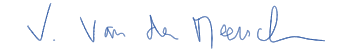
\includegraphics[scale=.65]{../../sign_long.png} \\
\noindent Victor Van der Meersch, PhD\\
\noindent \emph{Forest \& Conservation Sciences}\\
\noindent \emph{University of British Columbia}

\clearpage

\paragraph{References}
\printbibliography[heading=none]


\newpage

\end{document}


